%Zarantonello Umberto 2021-05-08

\section{Modelli Nucleari}
I modelli nucleari sono un tipo di supporto teorico che ci permette di interpretare le proprietà legate prima ai processi di decadimento e poi a quelli di fissione e fusione nucleare.
Come vedremo i modelli nucleari sono molto eterogenei e partono da presupposti che possono arrivare a contraddirsi.
Il modello a goccia per dire è opposto al modello di Fermi.
Questo esprime la difficoltà che si ha ad associare le proprietà dei nuclei a principi primi.
Quelli che introduciamo sono modelli fenomenologici o semi empirici, ciò indica che faremo delle supposizioni a partire da dati empirici per spiegare ciò che si vede.
Questo approccio è dovuto proprio alla mancanza di una teoria che con principi elementari esprima le proprietà dei nuclei.

%nuova sezione--------------------------------------------------
\subsection{Formula semi-empirica di massa}
Quello che verrà trattato in questa sezione riguarda quello che tiene legato il nucleo. 
Grazie all'esperimento di Rutherford sappiamo che il nucleo è formato da una carica positiva molto densa concentrata al centro, circondata poi da elettroni.
La cosa sorprendente di questa scoperta fu principalmente legata alla dimensionalità infatti, prima di Rutherford era logico pensare che la materia fosse densa, ma quello che ci rivelano i dati è appunto che tra il raggio nucleare e il raggio atomico c'è un fattore $10000$ che rende la materia di fatto "spazio vuoto".

\'E stato visto poi, con gli esperimenti di Rutherford e Chadwick, che il nucleo è composto da protoni e neutroni, in particolare con il nucleo può essere esplicitato con la formula
\begin{equation}
^{A}_{Z}X_{N}
\end{equation}
dove $X$ indica l'elemento, $A$ è il numero di massa, ovvero la somma di neutroni e protoni, $Z$ è il numero atomico, ovvero il numero di protoni e infine $N$ è il numero di neutroni ($A=Z+N$).
Si sa inoltre che la carica dell'atomo è assolutamente neutra e quindi che il numero di protoni è esattamente uguale al numero di elettroni.

\begin{figure}[h]
\centering
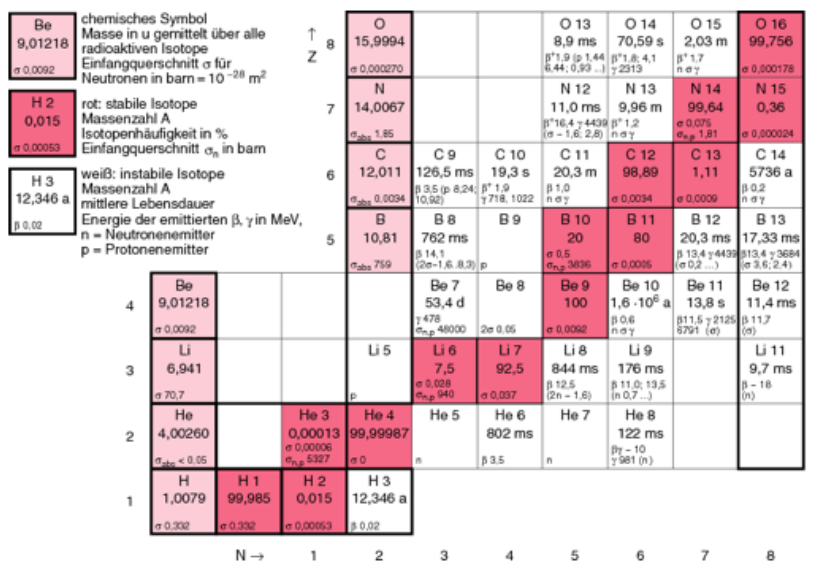
\includegraphics[width=300pt]{fig5_01}
\caption{Tavola dei Nuclidi}
\label{fig:5_01}
\end{figure}
La tavola dei nuclidi è uno strumento utile in fisica subatomica.
Sulla diagonale è rappresentata la linea degli elementi che possiedono un numero equivalente di neutroni e protoni.
Per numero di protoni bassi, i nuclidi che si trovano in natura, ovvero i nuclidi stabili, si trovano proprio lungo questa diagonale. 
Aumentando però il numero atomico i nuclidi stabili diventano quelli con un numero sempre maggiore di neutroni rispetto ai protoni.
Intorno a questa zona di nuclidi stabili vi è poi una zona di nuclidi instabili.
Oltre questa zona non vi sono poi più nuclidi, ne stabili ne instabili.

Cosa vuol dire atomo instabile?

Per nuclidi con protoni in eccesso, rispetto ai nuclidi stabili, ciò che accade è che l'atomo tende a decadere, ovvero uno o più protoni in eccesso subirà la reazione di decadimento $\beta^+$
\begin{equation}
p\longrightarrow n+e^+\nu_e
\end{equation}
Nei nuclidi che hanno esuberanza di neutroni, la reazione che avverrà riguarda i neutroni e si definisce decadimento $\beta^-$
\begin{equation}
n\longrightarrow p+e^- +\bar{\nu_e}
\end{equation}
(nelle formule sopra $p$ indica il protone, $n$ il neutrone, $e^-, e^+$ rispettivamente l'elettrone e il positrone, $\nu_e, \bar{\nu_e} $ il neutrino e l'antineutrino elettronici).

In questo tipo di trasformazioni si ha che la carica e il numero leptonico si conservano sempre. 
La carica è abbastanza evidente, per quanto riguarda il numero leptonico per ora ci basta sapere che viene conservato.

Com'è intuibile nel decadimento $\beta$ il nucleo si trasmuta variando il tipo di nucleo, solo che nel primo caso si ottiene un nuclide con un protone in meno dell'originale mentre nel secondo caso il nuclide avrà il numero dei protoni aumentato.
\begin{equation}
\begin{split}
\beta^+\hspace{0.5cm}^A_ZX \longrightarrow ^A_{Z-1}Y+e^+ +\nu_e\\
\beta^-\hspace{0.5cm} ^A_ZX \longrightarrow ^A_{Z+1}Y+e^- +\bar{\nu_e}
\end{split}
\end{equation}
Nella tavola dei nuclidi si avrà quindi che le reazioni provocheranno uno spostamento dell'elemento all'interno della tavola in diagonale (perpendicolarmente alla bisettrice del grafico).

Introduciamo ora il concetto di \emph{energia di legame}. 
Se supponiamo che all'interno di un nucleo ci siano Z protoni e N neutroni, prendendo la massa delle particelle libere che compongono il nucleo e confrontandola con la massa delle stesse particelle legate nel nucleo, si ottiene che quest'ultima è sempre minore della somma delle masse delle particelle libere.
Si ha quindi che parte della massa si trasforma in energia di legame, secondo la formula 
\begin{equation}
\Delta m c^2 \to BE
\end{equation}
La massa che va a formare il legame, chiamata massa mancante, è proprio la responsabile della diminuzione di massa nelle particelle legate rispetto alle particelle libere.

Calcoliamo ora per esempio l'energia che si ottiene trasformando un protone
\begin{equation}
p=10^{-27}kg\hspace{1cm} m_pc^2= 10^{-27}\cdot 9\times10^{16}\cdot 1,6\times10^{-19}\simeq 10^9 eV
\end{equation}

Qual è la differenza quindi tra massa legata e massa libera?
Per un atomo la massa costituente degli elementi degli atomi è
\begin{equation}
(Zm_p+Nm_n+Zm_e)c^2=m_{At}(^A_ZX)c^2+BE_{nuc}+BE_{at}
\end{equation}
dove $BE_{nuc}+BE_{at}$ corrispondono all'energia di legame nucleare e all'energia di legame atomica.
Si possono fare dei calcoli sulla formula sopra
\begin{equation}
Z(m_p+m_e)c^2+Nm_nc^2+Nm_nc^2=m_{At}(^A_ZX)c^2+BE_{nuc}+BE_{at}
\end{equation}
Siccome stiamo ragionando "sperimentalmente" per trovare un modo di calcolare la massa dei nuclei, noi conosciamo già l'energia di legame dell'atomo di idrogeno, per cui
\begin{equation}
m_{At}(^1_1H)c^2+B_{at}^H=m_p+m_e
\end{equation}
che sostituito porta a 
\begin{equation}
Z({m_{At}^1} {_1H c^4})+ZBE^H_{At}+Nm_nc^2=m_{At}(^A_ZX)c^2+BE_{nuc}+BE_{at}
\end{equation}
A questo punto posso notare che l'energia di legame dell'atomo di idrogeno e l'energia di legame dell'atomo si possono semplificare, ottenendo così l'energia di legame
\begin{equation}
BE_{nuc}=Z(m_{At}^1{_1Hc^4})+Nm_nc^2-m_{At}(^A_ZX)c^2
\end{equation}
Posso quindi misurare semplicemente l'energia di legame, infatti la massa dell'idrogeno è nota così come la massa del neutrone; basterà semplicemente misurare la massa dell'atomo legato.

\paragraph{Qual è la natura della forze che tengono insieme un nucleo?}
\'E chiaro che all'interno del nucleo ci debba essere una forza molto grande perché questo possa esistere, si deve infatti controbilanciare la forza elettrostatica di repulsione tra cariche uguali. 
Essendo che in natura esistono nuclei con numero atomico fino a 100 questa forza deve essere  almeno un fattore 100 rispetto alla forza elettrostatica.
Il modello che cerca di spiegare questa forza è appunto il \emph{modello a goccia}.

Ipotizziamo di avere una forza che agisce tra tutte le coppie di nucleoni, questo vuol dire che questa forza non distinguerà tra protoni e neutroni.
Siccome tra ogni coppi ci dovrà essere una forza procediamo a costruire il modello.
Tra tre particelle il numero di coppie possibili è 3, tra quattro particelle si formeranno 6 coppie. 
Si può quindi evidenziare una legge che stabilisce il numero di coppie in un nucleo con numero di massa $A$
\begin{equation}
\frac{A(A-1)}{2}=\frac{A^2-A}{2}
\end{equation}
Questo vuol dire che l'energia di legame totale del nucleo sarà proporzionale a $A^2$ e l'energia di ogni legame singolo sarà proporzionale a $A$.
\begin{equation}
BE\propto A^2\to \frac{BE}{A}\propto A
\end{equation}
Abbiamo quindi creato un'ipotesi che ora va verificata.
Se quest'ipotesi fosse vera si avrebbe che $BE/A$ e $A$ devono risultare proporzionali e aumentare linearmente l'uno rispetto all'altro.
I dati sperimentali ci dicono in realtà che l'energia di legame aumenta quasi linearmente fino ad un massimo (coincidente con il ferro $^{56}Fe$) e che dopo si stabilizza ad un valore $\sim 8MeV$ rimanendo circa costante all'aumentare di A.
\begin{figure}[h]
\centering
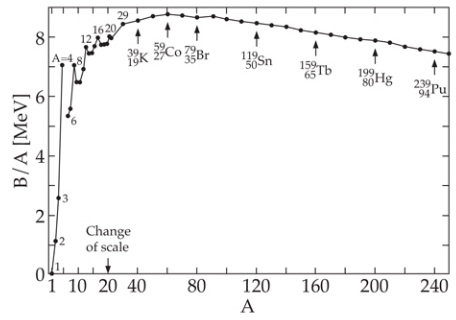
\includegraphics[width=180pt]{fig5_04}
\caption{Grafico sperimentale  dell'energia di legame in funzione con l'aumento del numero di massa}
\end{figure}

Questo errore deriva dal fatto che abbiamo supposto che i nucleoni interagiscano infinitamente anche con i nucleoni più distanti, questo è stato dimostrato non essere vero e anzi che si raggiunge una saturazione.

Si ha quindi che due nucleoni lontani non si parlano.
La forza nucleare è dunque una forza a corto range.

Abbiamo imparato che l'energia di legame (\emph{Bending energy}) corrisponde a 
\begin{equation}
BE=a_vA
\end{equation}
dove $a_v$ è un termine di volume.

Questa formula avrà intuitivamente una serie di termini correttivi. 
Una prima correzione è dovuta al fatto che sicuramente i nucleoni centrali avranno più legami rispetto ai nucleoni sulla superficie della sfera (da qui deriva il nome di modello a goccia, infatti si basa sulla stessa struttura delle gocce di acqua).
Continuando ad approssimare devo tener conto di un termine di superficie che diminuisce l'energia di legame.
\begin{equation}
BE=a_vA-a_sA^{2/3}
\end{equation}
$A^{2/3}$ esprime la dipendenza dalla superficie perché il raggio nucleare ha formula
\[
R=R_0A^{1/3}
\]
e la superficie della sfera è
\[
S=4\pi R^2
\]
il che restituisce una proporzionalità di superficie di $A^{2/3}$.

Il terzo termine deriva dal fatto che all'interno del nucleo sono presenti i protoni che possiedono una forza di repulsione elettrostatica tra loro
\[
F_Q=\frac{Q_1Q_2}{4\pi \varepsilon_0 R^2}
\]
In realtà ciò che interessa a noi è l'energia potenziale.
\[
PE\propto \frac{1}{R}=\frac{K}{A^{1/3}}
\]
Il termine coulombiano della forza di legame è quindi
\begin{equation}
=a_c\frac{Z(Z-1)}{A^{1/3}}
\end{equation}
Aggiungendo questo termine si trova che l'energia di legame è
\begin{equation}
BE=a_vA-a_sA^{2/3}-a_c\frac{Z(Z-1)}{A^{1/3}}
\end{equation}

Perché la formula dell'energia di legame sia completa mancano altri due termini.
Mentre tutti i termini trovati fino ad ora si possono considerare come termini classici gli ultimi sono termini puramente quantistici. 

Il primo è legato al fatto che i protoni e i neutroni possono essere descritti come intrappolati in una buca di potenziale.
All'interno di una buca di potenziale i livelli sono quantizzati e soprattutto equispaziati.
Supponiamo che esistano due buche di potenziale, una dei protni e una dei neutroni, all'interno di questa buca i nucleoni si dispongono con spin antiparallelo.
Continuando ad aggiungere neutroni nella buca e superando il numero di protoni io avrò che mi ci vuole meno energia per estrarre un neutrone, in quanto avranno occupato dei livelli energetici più alti dei protoni (sono meno fortemente legati).
Questo eccesso di energia corrisponde a 
\begin{equation}
E= 2S+ 2(2S)+2(3S)+ ...+ 2(\frac{X}{2}S)
\end{equation}
dove $S$ è la differenza energetica tra i livelli che viene moltiplicato per il numero di livelli in eccesso, $X$ è infatti l'eccesso di neutroni ovvero $X=N-Z$.
Quella sopra è evidentemente una serie geometrica che da come somma
\begin{equation}
E=2S\biggl[\frac{X}{2}\biggl(\frac{X}{2}+1\biggl]/2=S\biggl(\frac{X^2}{4}+\frac{X}{2}\biggl)
\end{equation}
Se X è grande portò ignorare il termine $X/2$.
Se $A$ aumenta ciò che succede è che non  aumento il livello massimo occupato all'interno della buca ma diminuisce la spaziatura tra i livelli stessi
\begin{equation}
A\uparrow \rightarrow S\downarrow \rightarrow S\propto \frac{1}{A}
\end{equation}
Quindi 
\begin{equation}
S\frac{X^2}{4}\propto \frac{1}{A}(N-Z)^2
\end{equation}
Il termine che si andrà ad aggiungere alla formula di legame nucleare definito anche termine di simmetria sarà
\begin{equation}
a_{sym}\frac{(N-Z)^2}{A}
\end{equation}
La formula aggiornata sarà ora
\begin{equation}
BE=a_vA-a_sA^{2/3}-a_c\frac{Z(Z-1)}{A^{1/3}}-a_{sym}\frac{(N-Z)^2}{A}
\end{equation} 

L'ultimo termine che manca è legato al fatto che i nucleoni tendono ad accoppiarsi con spin antiparallelo e quindi risulta che i nuclei con numero di nucleoni pari saranno più legati rispetto a quelli con numero negativo.
Nella tabella sono raffigurati i valori che può assumere l'ultimo termine di correzione in base al numero di nucleoni che sono presenti nel materiale.
\begin{figure}[h]
\centering
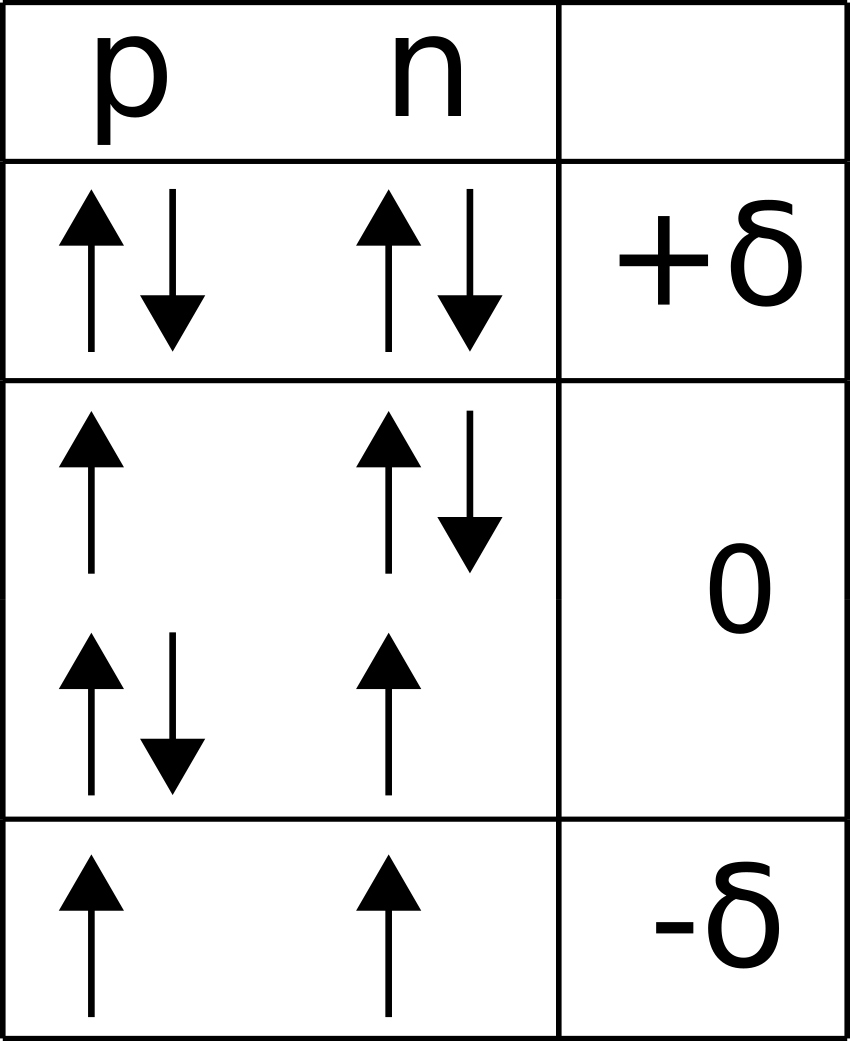
\includegraphics[width=120pt]{fig5_02}
\end{figure}

La formula finale ottenuta è quindi
\begin{equation}
BE=a_vA-a_sA^{2/3}-a_c\frac{Z(Z-1)}{A^{1/3}}-a_{sym}\frac{(N-Z)^2}{A}+\delta
\end{equation}

Ora possiamo finalmente calcolare la massa del la massa del nucleo
\begin{equation}
\begin{split}
m_{nucl} ^A-Z X c^2 &=Z m_p c^2+N m_n c^2- BE_{nucl} \\
&=Zm_pc^2+Nm_nc^2-\biggl[ a_v A-a_s A^{2/3}-a_c \frac{Z(Z-1)}{A^{1/3}}-a_{sym}\frac{(N-Z)^2}{A}+\delta \biggl]
\end{split}
\end{equation}
Questa formula è quella che viene chiamata formula semi-empirica di massa.
\'E una formula empirica in quanto deriva da valori sperimentali ma non lo è totalmente in quanto sono stati inseriti pure vari termini determinati con la teoria.
Ciò che non abbiamo ancora specificato sono i valori dei termini moltiplicativi. 
Questi possono variare in base ai testi o ai fit da cui sono derivati, ogni set di valori possiede numeri consistenti tra loro.
\begin{equation}
\begin{split}
a_v &=15,8MeV\\
a_s&=18,3MeV\\
a_c&=0,714MeV\\
a_{sym}&=23,2MeV\\
\delta=33,5MeV
\end{split}
\end{equation}
\begin{figure}[h]
\centering
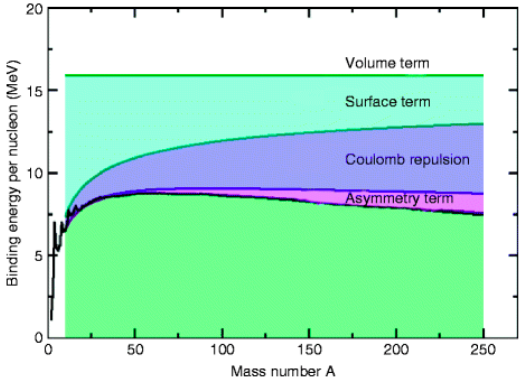
\includegraphics[width=180pt]{fig5_03}
\caption{Modifiche all'energia di legame date da ogni termine}
\end{figure}

\paragraph{Limiti alla creazione dei nuclei}
La domanda a cui risponderemo in questo paragrafo è "perché non posso creare le combinazioni che voglio di portoni e neutroni ma solo alcune sono ammesse?".
La risposta molto semplicemente è che la natura richiede che si minimizzi l'energia di massa.

Prendendo quindi la formula semi-empirica di massa e derivandola rispetto a $Z$ ottengo
\begin{equation}
\frac{dM}{dZ}=m_pc^2-m_nc^2-0-0+a_c\frac{2Z-1}{A^{1/3}}+a_{sym}\frac{[-4A+8Z]}{A}
\end{equation}
Ponendo questo differenziale uguale a zero ottengo la condizione richiesta di minimizzare la massa (siccome la massa di neutrone e protone sono circa uguali i due termini di massa si elidono)
\begin{equation}
Z\left(\frac{2a_c}{A^{1/3}}+\frac{8a_{sym}}{A}\right)=\frac{a_c}{A^{1/3}}+4a_{sym}
\end{equation}
Ciò che cerco di ricavare ora è $Z$ che corrisponde al valore di Z che minimizzi la massa
\begin{equation}
Z=\frac{\frac{a_c}{A^{1/3}}+4a_{sym}}{\frac{2a_c}{A^{1/3}}+\frac{8a_{sym}}{A}}
\end{equation}
Questa formula mi restituisce quindi per ogni $A$ il valore di $Z$ che minimizza la massa.
La formula finale è
\begin{equation}
Z=\frac{A}{2}\biggl[\frac{1}{1+0,008A^{2/3}}\biggl]
\end{equation}
Si deduce che se A è piccolo allora $Z=A/2$ e quindi $N=Z$, mentre se A è grande allora $N>Z$.
Intuitivamente questo serve a bilanciare la repulsione elettrostatica dei nuclei con alto numero di protoni.

Studiamo ora gli andamenti che si possono ottenere dalla formula semi-empirica di massa.
Questa formula si può vedere come un polinomio del tipo
\begin{equation}
M=a+ bZ +cZ^2
\end{equation}
Fissato A, la casistica a questo punto si divide in due, i nuclei che hanno numero di massa dispari e quelli con numero di massa pari.

Il caso più semplice si ha per A dispari.
\begin{figure}[h]
\centering
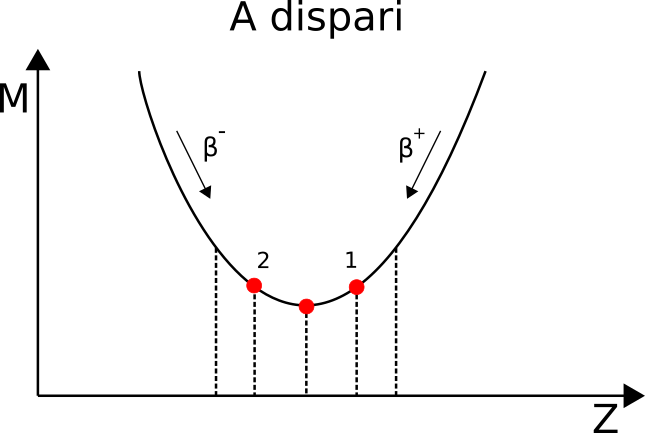
\includegraphics[width=180pt]{fig5_05}
\caption{rappresentazione delle masse possibili al variare di Z con A pari}
\end{figure}
In figura sono rappresentati degli stati possibili con A dispari, lo stato centrale è quello a massa minima e quindi anche quello più stabile.
Procedendo verso lo stato 1 si troveranno i nuclei con un eccesso di protoni mentre al contrario procedendo verso 2 quelli con eccesso di neutroni.
Ciò comporta che 2 avrà la tendenza a decadere nello stato centrale con decadimento  $\beta^-$ mentre 1 decadrà naturalmente con decadimento $\beta^+$.
Nei punti in cui  la parabola assume valori troppo elevati non si ha la presenza di stati.

Nel caso di A pari la faccenda si complica in quanto le parabole possibili sono due, una ad energia più alta e che corrisponde al caso di numero di protoni e neutroni entrambi dispari(Odd-Odd: come già visto sopra questo genera nuclei più instabili) e una a numero di neutroni e protoni pari ad energia più bassa (Even-Even:  quindi con nuclei più stabili).
Si ha quindi la possibilità di avere lo stato centrale o su una parabola o sull'altra portando a due casistiche differenti.
\begin{figure}
\centering
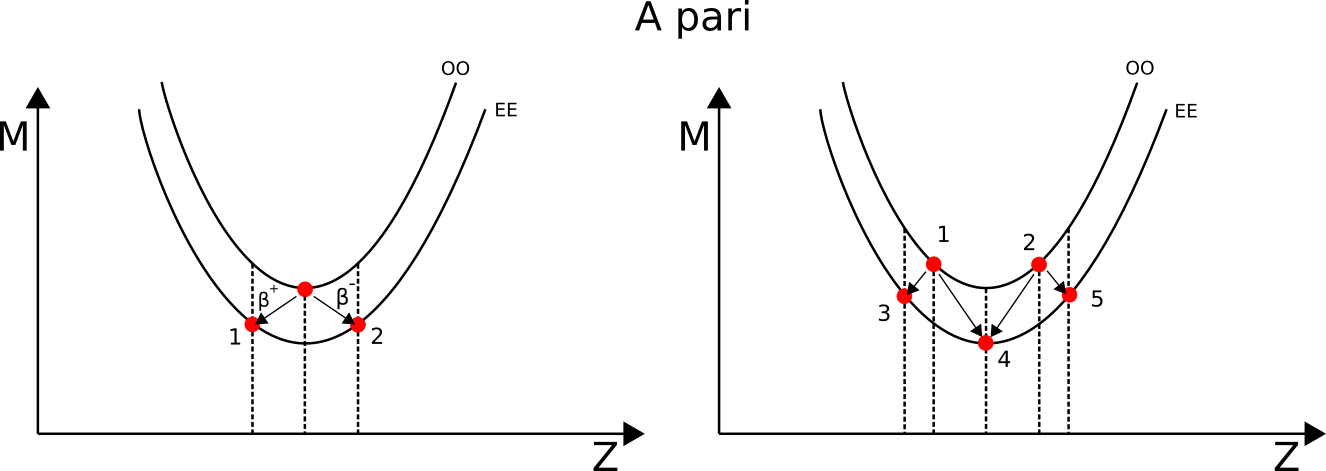
\includegraphics[width=380pt]{fig5_06}
\caption{rappresentazione delle masse possibili al variare di Z con A dispari}
\end{figure}

Nel grafico a sinistra possiamo notare che gli stati stabili sono due in quanto lo stato centrale si trova sulla parabola superiore mentre sulla parabola inferiore sono presenti due stati sullo stesso livello di energia e quindi entrambi con la stessa stabilità. 
Lo stato superiore in questo caso ha due possibilità di decadimento, verso 1 con decadimento $\beta^+$ o verso 2 con decadimento $\beta^-$.
Nel caso per dire che lo stato 1 fosse più elevato di 2, la transizione da 1 a 2 non è impossibile ma altamente improbabile, in quanto pur essendo energeticamente favorevole richiederebbe un secondo decadimento $\beta$ che richiede quindi una seconda probabilità di avvenimento.
Un processo di questo tipo si chiama decadimento \emph{doppio $\beta$}.

Nel grafico a destra è invece mostrato il caso in cui si abbia il nucleo centrale e nella curva più bassa (4), nella curva superiore vi sono invece due nuclei ad energia uguale.
I nuclei 1 e 2 come si vede nel grafico avranno due possibilità di decadimento ciascuno, verso 3,4 e 5.
Come nel caso precedente i decadimento da 3 e 5 verso 4 pur essendo energeticamente favorevoli sono improbabili in quanto decadimenti doppio $\beta$. 
I nuclei 3,4 e 5 sono quindi considerati tutti nuclei stabili.

La zona in cui non si ha la generazione di nuclei, sia provocata da un eccesso di neutroni che di protoni è dovuta al fatto che non è energeticamente favorevole avere nuclei piuttosto che le particelle slegate o un nucleo con numero di massa inferiore e delle particelle libere. 
\begin{equation}
\begin{split}
^A_ZX &\longrightarrow ^{A-1}_ZX+n\\
^A_ZX &\longrightarrow ^{A-1}_{Z-1}Y+p
\end{split}
\end{equation}
Se infatti la somma delle masse slegate a destra delle due reazioni sopra risulta minore della massa dell'atomo legato a sinistra la natura tenderà a dividere il nucleo.
Per lo stesso principio i nuclei che sono troppo pesanti ovvero che possiedono semplicemente troppi nucleoni tenderanno ad emettere particelle $\alpha$; questo tipo di nuclei sono anche quelli che fanno la fissione nucleare ovvero che tenderanno a dividersi in due atomi a numero di massa inferiore.

%nuova sezione--------------------------------------------------
\subsection{Modello di Fermi}
Questo modello a differenza di quello a goccia è un modello a particella singola, ovvero studia l'interazione di una particella con un potenziale generato dalle altre particelle piuttosto che vedere il sistema in generale come insieme di particelle.
Questo perché i sistemi complessi sono difficili da calcolare e inoltre quasi mai si riesce a risolvere i calcoli in maniera analitica.
Il modello di Fermi suppone che il nucleo è composto da due gas di fermioni, protoni e neutroni.
I fermioni sono le particelle che soddisfano alla statistica di Fermi-Dirac, che afferma che due particelle non possono occupare lo stesso stato quantico.
Il risultato di questa ipotesi iniziale sarà poi confermato dal modello.
Trascuriamo l'interazione tra le singole particelle ma le consideriamo confinate in una buca di potenziale che ha delle dimensioni del nucleo.
Questo potenziale è dato dall'interazione media con tutte le altre particelle, quindi in realtà il modello considera le iterazioni ma le approssima ad un potenziale generato proprio da tali  interazioni.
La buca di potenziale che confina i due gas è quindi generata dai gas stessi.
Questa impostazione ci permetterà di fare delle ipotesi sulle proprietà che i nucleoni hanno all'interno del nucleo.
Questo modello fa inoltre parte dei così-detti modelli a particelle indipendenti.

Supponiamo di avere due buche di potenziale, in quanto neutroni e protoni sono considerati particelle indipendenti quindi ognuno avrà la propria buca.
La buca di potenziale dei protoni è meno profonda in quanto questi subiscono anche la repulsione coulombiana, questo ci fa capire un po' di più sul modello a goccia, se ricordiamo infatti si aveva che i nuclei più pesanti possedevano più neutroni a livello di stabilità, proprio a causa di questa repulsione.

Questo modello prevede che sia per i neutroni che per i protoni vi siano dei livelli energetici, occupati fino ad un livello massimo che è il \emph{livello di Fermi}.
Per ogni livello energetico posso sistemare al massimo due particelle con spin opposto,questo per il principio di esclusione di Pauli.

I parametri che caratterizzano questo sistema sono la profondità della buca di potenziale e il livello di Fermi (livello energetico più alto occupato).

Siccome i nucleoni nel nucleo non sono particelle relativistiche possono essere descritti con la meccanica quantistica non relativistica, ovvero quella che viene fatta nella triennale.
Si possono quindi sfruttare le equazioni di Schroedinger.
Vogliamo risolvere l'equazione per una buca di potenziale con energia potenziale
\begin{equation}
\begin{split}
E_{pot} &=V_0\hspace{0.5cm}r\leq a\\
&=0\hspace{0.5cm}r>a
\end{split}
\end{equation}
L'equazione di Schroedinger è indipendente dal tempo e corrisponde a
\begin{equation}
-\frac{\hbar^2}{2m}\frac{d^2}{dr^2}\psi+V_0\psi=E
\end{equation}
La risoluzione è
\begin{equation}
\frac{d^2}{dr^2}\varphi=-\frac{2m}{\hbar}(E-V_0)\varphi
\end{equation}
Per risolverlo bisogna notare che il termine 
\[
-\frac{2m}{h}(E-V_0)>0
\]
Perché $V_0$ è un'energia potenziale di confinamento e una buca di potenziale ha potenziale negativo ($V_0$ è un potenziale attrattivo. 
Quindi posso sostituire il tutto con una variabile reale positiva ottenendo
\begin{equation}
\frac{d^2}{dr^2}\psi+K^2\psi=0 \hspace{0.5cm} K=\sqrt{\frac{2m(E-V_0}{\hbar^2}}
\end{equation}
La soluzione (identica a quella del moto armonico) è
\begin{equation}
\psi=A\sin Kr+B\cos Kr
\end{equation}
A cui devo poi porre le condizioni di annullamento in $0$ e $a$.
\begin{equation}
\begin{split}
&\psi(0)=0\to B=0\hspace{1cm}\psi=A \sin Kr\\
&\psi(a)=0\to Ka=n\pi \to K=n\frac{\pi}{a}\\
&\to E=\frac{p^2}{2m}=\frac{\hbar^2K^2}{2m}=\frac{\hbar^2}{2m}\frac{\pi^2}{a^2}n^2
\end{split}
\end{equation}
Questi sono quindi i livelli energetici consentiti all'interno della buca di potenziale, le funzioni d'onda corrispondenti saranno come in figura.
\begin{figure}[h]
\centering
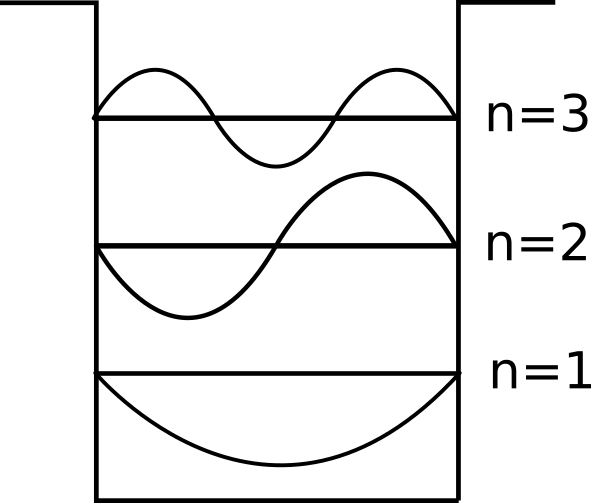
\includegraphics[width=120pt]{fig5_07}
\end{figure}
Se la buca non fosse finita ci sarebbe un'estensione delle funzioni d'onda oltre le pareti della buca.

\paragraph{Stima della profondità della buca di potenziale} Per capire la profondità della buca dobbiamo valutare il numero di stati nucleari nello spazio delle fasi in un volume $V$ e con quantità di moto $p$.
Lo spazio delle fasi è uno spazio a 6 dimensioni che comprende sia le coordinate spaziali che quelle riferite alla quantità di moto nelle tre direzioni. 
Per capire, è un unico spazio a 6 dimensioni che mi dice proprio l'estensione del sistema che sto studiando, quindi qual è lo spazio delle fasi occupato dal gas di neutroni e protoni.
Il numero di nucleoni in funzione di $p$ è dato da
\begin{equation}
dn(p)=\frac{V4\pi p^2 dp}{(2\pi\hbar)^3}
\end{equation}
dove $V$ è il volume nelle coordinate spaziali, $4\pi p^2dp$ è un guscio sferico compreso tra la sfera di raggio $p$ e la sfera $p+dp$, $(2\pi \hbar)^3$ è lo spazio delle fasi occupato da ognuno degli stati quantici, in pratica è un volume di dimensione $\hbar$, quest'ultima quantità è legata al principio d'indeterminazione $\Delta p\Delta x \sim h$ (ogni stato quantico occupa dello spazio delle fasi un volume pari ad $\hbar^3$).
Per calcolare il numero totale di stati devo integrare sapendo che il volume del nucleo è
\[
V=\frac{4}{3}\pi R^3\hspace{0.5cm}R=R_0A^{\/3}
\]
Il numero totale di nucleoni sarà dunque
\begin{equation}
\begin{split}
n &=2\int^{p_F}_0 n(p) dp=\frac{2V4\pi}{(2\pi \hbar)^3}\int_0^{p_F}pdp\\
&=\frac{V}{\pi^2\hbar^3}\biggl[\frac{p_F}{3}\biggl]
\end{split}
\end{equation}
Questo è valido sia per i protoni che per i neutroni, anche se poi soddisfano indipendentemente a due statistiche diverse.
\begin{equation}
N=\frac{V}{3\pi^2\hbar^3}(p^n_F)^3\hspace{1cm}Z=\frac{V}{3\pi^2\hbar^3}(p^p_F)^3
\end{equation}
Ora per semplificarci la vita consideriamo un nucleo con $N=Z=A/2$.
Questo non cambierà le considerazioni finali.
Ciò che si ottiene è
\begin{equation}
\begin{split}
&p_F^3=\frac{A}{2}\frac{3\pi^2\hbar^3}{\frac{4}{3}\pi R_0^3A}\\
&\to p_F=\frac{\hbar}{R_0}\left(\frac{9\pi}{8}\right)^{1/3}=250\frac{MeV}{fm}
\end{split}
\end{equation}
Dato il momento di Fermi possiamo ricavare anche l'energia di Fermi
\begin{equation}
E_F=\frac{p^2}{2M}= \frac{(250MeV/c)^2}{2\times940MeV/c^2}\approx33MeV
\end{equation}
Questa energia rappresenta l'ultimo livello occupato del nucleone ma non corrisponde alla profondità della buca di potenziale, per ottenere questa altezza è necessario infatti sommare all'energia di Fermi l'energia di legame media per nucleone corrispondente a $\sim7MeV$.
Si ha quindi che il potenziale nonchè la profondità della buca è pari a 
\begin{equation}
V_0=33+7 MeV=40MeV
\end{equation}
Questo modello è uguale a quello degli elettroni nel metallo ma le grandezze sono più piccole ($\sim10eV$).
Da notare che questa è la buca di potenziale per nuclei con numero qualsiasi di nucleoni, l'energia di Fermi è quindi sempre uguale ma ciò che cambia sarà la spaziatura tra i livelli che diventa più piccola nel caso di nuclei pesanti.

\paragraph{Considerazioni}
Con questo modello si riescono a spiegare i nuclei più semplici.
\begin{itemize}
\item Un argomento che si può esemplificare con il modello a gas di Fermi è per dire la nucleosintesi primordiale.
Nei primi minuti dell'universo si sono sintetizzati l'idrogeno e l'elio ma per gli elementi più pesanti si è dovuto attendere 200 milioni di anni e la sintesi delle prime stelle.
Questo immenso gap temporale Si può spiegare grazie a questo modello.
Nelle buche di potenziale infatti l'elio 4 è composto da due neutroni e due protoni.
\begin{equation}
^4_2He_2\hspace{1cm}2n+2p
\end{equation}
In questa configurazione il nucleo è estremamente stabile, se si avesse però un quinto nucleone (protone o nucleone) questo andrebbe ad occupare un livello energetico più alto.
\begin{figure}[h]
\centering
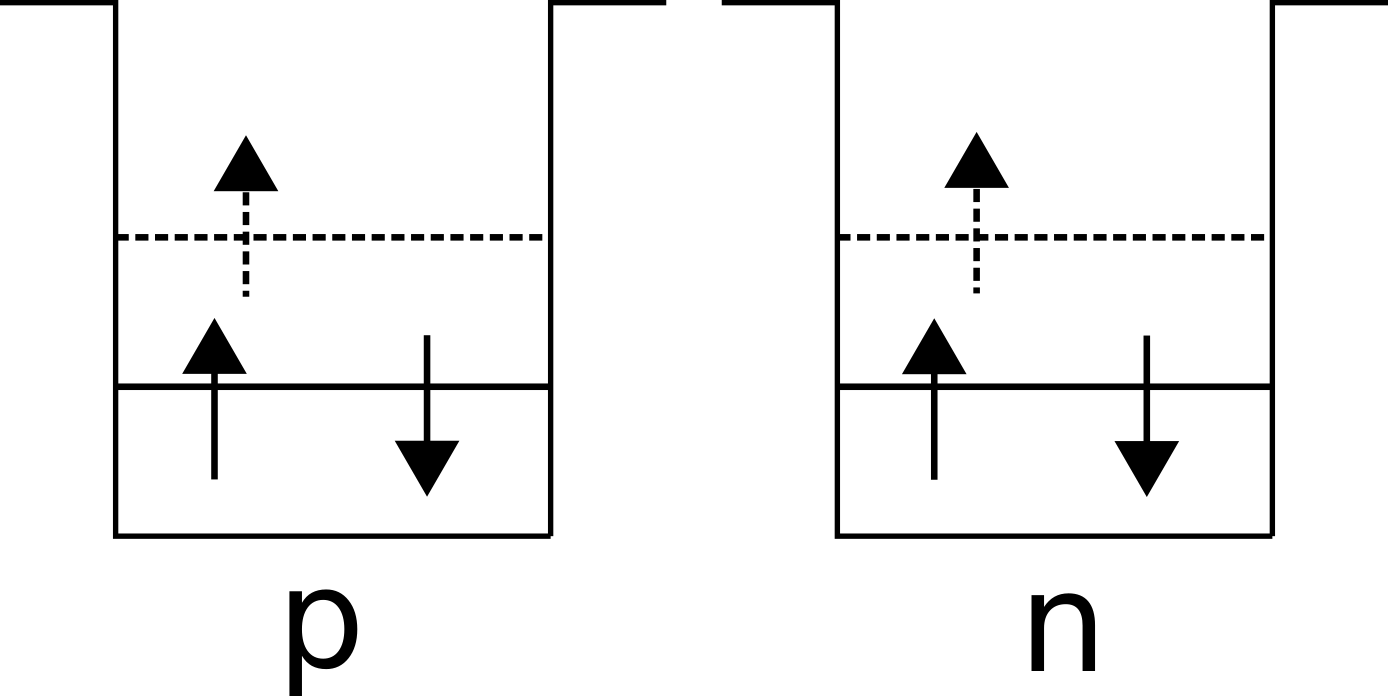
\includegraphics[width=150pt]{fig5_08}
\end{figure}

Quello che la natura ci mostra è però che non esistono nuclei stabili con numero di massa pari ad $A=5$.
Vuol dire che semplicemente la nucleosintesi degli elementi si è fermata all'elio, se fosse esistito un terzo elemento l'evoluzione dell'universo sarebbe stata molto diversa.

\item Un altro effetto spiegabile è il decadimento$\beta$, in particolare il motivo per cui il protone risulta stabile fuori dal nucleo ma può decadere nel caso sia all'interno del nucleo.
Ricordiamo ancora i decadimenti $\beta$
\begin{equation}
\begin{split}
\beta^-:\hspace{0.2cm}n\longrightarrow p+e^-+\bar{\nu_e}\\
\beta^+:\hspace{0.2cm}p\longrightarrow n+e^++\nu_e
\end{split}
\end{equation}
Questo vuol dire semplicemente continuando a mettere protoni oltre il numero di neutroni otterrò nel livello dei neutroni un livello libero e questo causa il decadimento.
\begin{figure}[h]
\centering
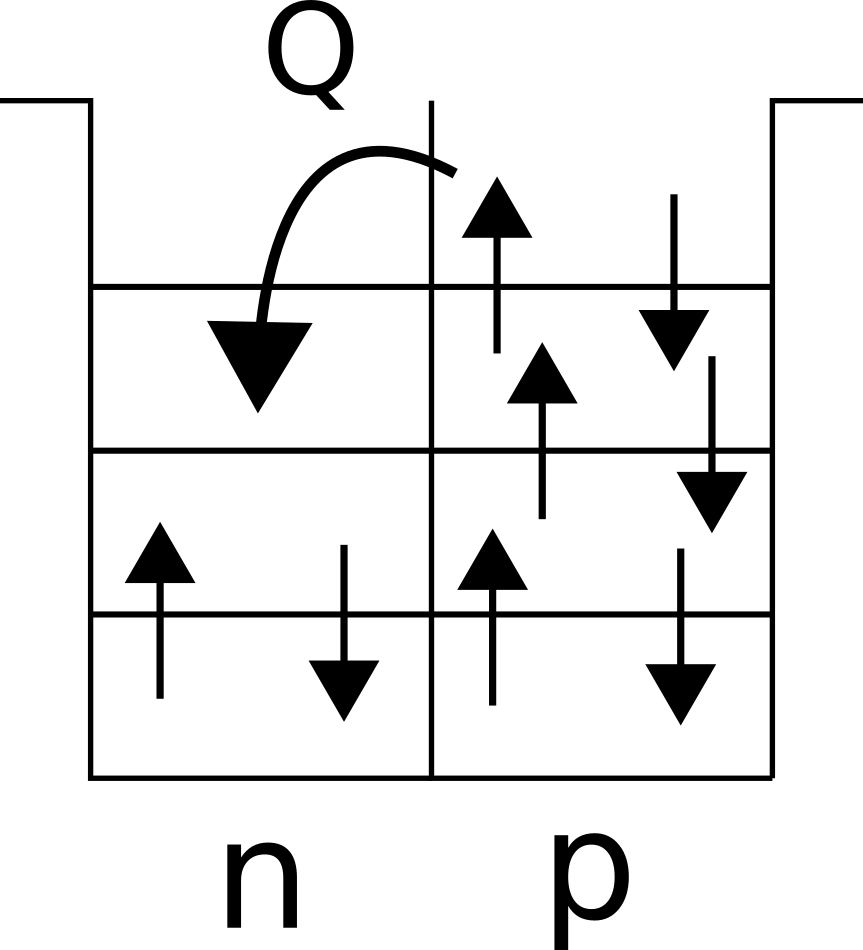
\includegraphics[width=120pt]{fig5_09}
\caption{Decadimento del protone nel nucleo}
\end{figure}

Al di fuori del nucleo non può avvenire in quanto il $Q=M_i-M_f$ della reazione non è favorevole (è negativo), ovvero l'energia di massa del protone fuori dal nucleo è minore dei prodotti della reazione mentre all'interno del nucleo la questione è opposta.
\begin{equation}
\beta^+\hspace{0.2cm}Q=m_p-m_n-m_{e^+}-m_\nu
\end{equation}
Riportiamo quindi le masse del decadimento 
\begin{equation}
\begin{split}
&m_p=938,2\frac{MeV}{c^2}\\
&m_n=939,5\frac{MeV}{c^2}\\
&m_e=0,511\frac{MeV}{c^2}
\end{split}
\end{equation}
Il $Q$ della reazione risulta quindi essere in questo caso
\begin{equation}
Q^{\beta^+}=-1,8MeV
\end{equation}
Questa è una reazione endotermica e quindi non avviene spontaneamente.
Il $Q$ del decadimento del neutrone fuori dal nucleo è invece
\begin{equation}
Q^{\beta^-}=m_n-m_p-m_{e^-}=0,8MeV
\end{equation}
Il neutrone è stabile all'interno del nucleo per il principio di esclusione di Pauli che ne impedisce il decadimento, si ha però, come per il protone, che un eccesso di neutroni porta comunque al decadimento.

\item Nel modello a goccia abbiamo calcolato il libero cammino medio del nucleone nel nucleo corrispondente a $l=0,21fm$.
Nel modello di Fermi invece abbiamo considerato i nucleoni come un gas di particelle libere nel nucleo cioè prive di interazioni.

Queste due visioni apparentemente contrastanti si conciliano in quanto se non ci sono stati liberi le particelle non collidono tra loro (una collisione comporta uno scambio di energia che nella stabilità non vi può essere), quindi non è propriamente vero che il libero cammino medio è una frazione di Fermi poiché  con tutti gli stati occupati le particelle devono considerarsi libere.
\end{itemize}

%nuova sezione--------------------------------------------------
\subsection{Modello a shell}
L'evidenza sperimentale che portò alla costruzione di questo modello si basa sull'analogia con il modello a shell elettroniche dell'atomo. 
Facendo un grafico dell'energia di estrazione di un nucleone in funzione del numero atomico, si vide che aveva lo stesso andamento del grafico del lavoro di estrazione degli elettroni.
Sorge spontaneamente il dubbio che quindi possa avere una struttura a shell pure il nucleo.
\begin{figure}[h]
\centering
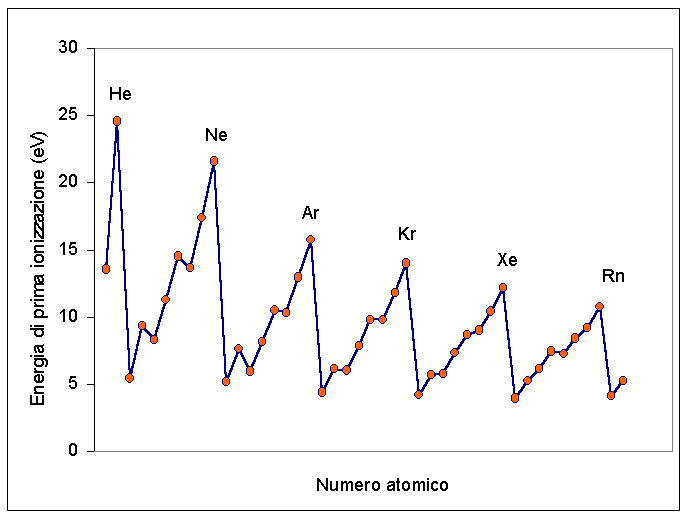
\includegraphics[width=150pt]{fig5_10}
\caption{Lavoro di estrazione elettronico in funzione del materiale}
\end{figure}

Ci sono un paio di differenze tra il modello elettronico e nucleare
\begin{itemize}
\item La prima consiste nell'ordine di grandezza, infatti, mentre per gli elettroni si parla di $eV$ nel caso dei nuclei di $MeV$, consistentemente con quanto già visto.

\item Il secondo è la posizione dei picchi.
Nel caso degli elettroni i picchi corrispondo ai gas nobili, nel caso dei nuclei i picchi corrispondono a 2, 8, 20, 28, 50, 82, 126 (si fa riferimento sia al numero di neutroni che di protoni).
Per esempio con il 20 si può avere il Calcio 40 $^{40}_{20}Ca$.
\end{itemize}

Ciò che non fu subito chiaro è come mai si hanno questi valori di massimo, infatti la struttura dell'atomo rende abbastanza evidente il motivo (regola dell'otteto e livelli energetici delle shell), mentre nel nucleo non c'è un potenziale ben definito che vada a creare dei livelli energetici così chiari in quanto ogni nucleone interagisce con gli altri (e come visto dal modello a goccia con un numero di legami differente).

Per risolvere questo problema bisogna considerare un nucleone e approssimare le interazioni con un potenziale medio.
\begin{figure}[h]
\centering
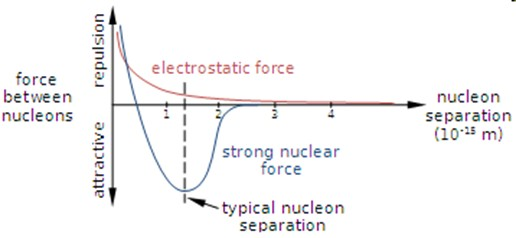
\includegraphics[width=150pt]{fig5_11}
\caption{Potenziale nucleare in funzione del raggio}
\end{figure}

Come si può vedere dal grafico il potenziale nucleare dovrà avere una forma in cui a valori molto bassi di raggio non implode su se stesso, e quindi valore positivo (potenziale repulsivo) ma che poi scende per creare una buca di potenziale negativa che arriva ad azzerarsi quando il raggio è pari al raggio nucleare, il tutto restando sempre in opposizione al potenziale elettrostatico.
Per approssimare questa forma si usa il potenziale di Saxon-Woods dove la forza repulsiva iniziale viene ignorata e la forma è a metà tra la curva e una buca di potenziale rettangolare.
\begin{figure}
\centering
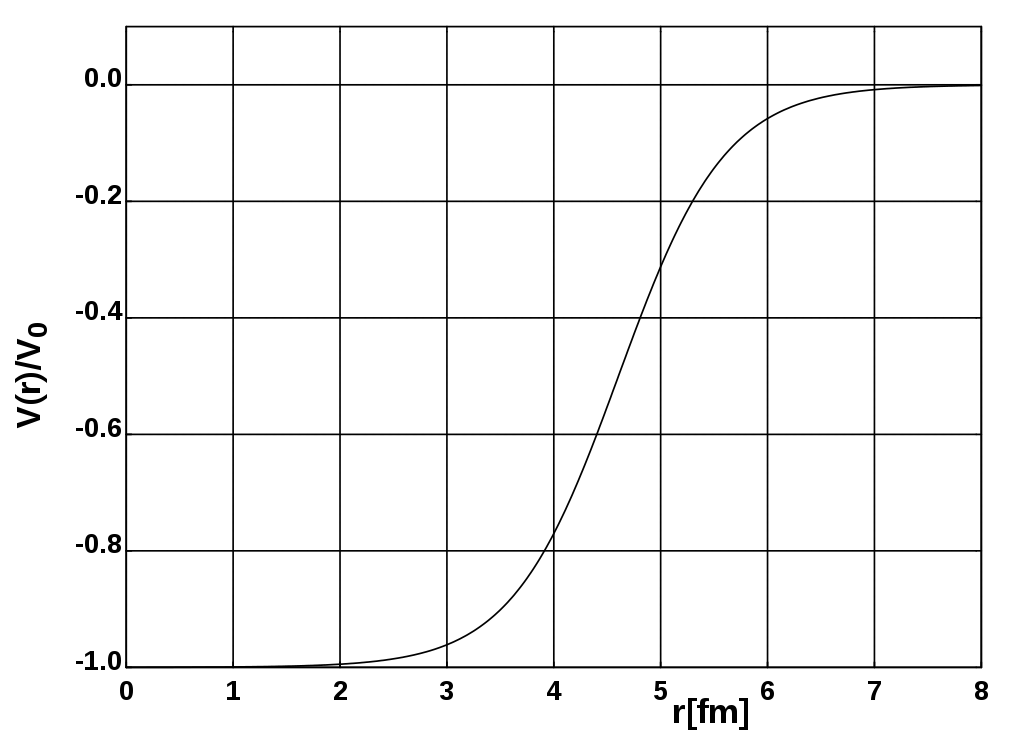
\includegraphics[width=150pt]{fig5_12}
\caption{Potenziale di Saxon-Woods}
\end{figure}

Il potenziale di Saxon-Woods ha formula
\begin{equation}
V=-\frac{V_0}{1+\frac{\exp(r-R)}{a}}
\end{equation}
Dove $V_0=50MeV$, $R=R_0A^{1/3}$ e $a=0,56fm$.

In particolare questo potenziale si differenzia dalla buca di potenziale classica nella regione tra i $3fm$ e i $7fm$ ed è proprio questa regione che determina le caratteristiche dei livelli energetici del nucleo.
\paragraph{Livelli atomici}
I livelli atomici sono caratterizzati da 4 numeri quantici: n, L, m, s.
\begin{equation}
\begin{split}
&\forall n\\
&l=0\to n-1\\
&m\hspace{0.5cm}-l<m<l\\
&s=\pm 1/2
\end{split}
\end{equation}
Le shell atomiche si formano quindi come
\begin{equation}
\begin{split}
n=1\hspace{0.5cm}&l=0\hspace{0.2cm}m_s=0\hspace{0.2cm}s=\pm 1/2\\
n=2\hspace{0.5cm}&l=0\hspace{0.2cm}m_s=0\hspace{0.2cm}s=\pm 1/2\\
&l=1\hspace{0.2cm}m=-1,0,+1\hspace{0.2cm}s=\pm1/2
\end{split}
\end{equation}
Si ha quindi che nel livello corrispondente a $n=1$ si possono avere solo 2 elettroni, mentre nel caso di $n=2$ posso avere 2 elettroni nel livello $l=0$ ma anche 6 nel livello $L=1$ il che mi porta ad avere 8 elettroni totali nel livello $n=2$.
Continuando intuitivamente si vede che per esempio il livello $n=3$ ospiterà 18 elettroni.
Questo restituisce esattamente le configurazioni dei primi 3 gas nobili corrispondenti a $Z=2,10,28$ ovvero i primi tre livelli completi.

Nei nuclei abbiamo visto che questi valori non coincidono con i livelli elettronici infatti i valori sono $Z=2, 8, 20, 28, 50, 82, 126$.
Questo è dovuto al fatto che nei nuclei $l$ non è limitato a $n-1$ e inoltre i nuclei hanno la tendenza ad accoppiare lo spin e il momento angolare introducendo un momento 
\[
j=L+s
\]
che può assumere i valori 
\[
j=1/2, 3/2, 5/2, 7/2, \dots
\]
Si ottiene così che il numero di nucleoni in funzione di $j$ sarà
\begin{equation}
\begin{split}
&j\hspace{0.5cm}n\\
&\frac{1}{2}\hspace{0.5cm}2\\
&\frac{3}{2}\hspace{0.5cm}4\\
&\frac{5}{2}\hspace{0.5cm}6\\
&\frac{7}{2}\hspace{0.5cm}8
\end{split}
\end{equation}
La regola generale è quindi
\begin{equation}
j=\frac{X}{2}\longrightarrow n=X+1
\end{equation}
La nomenclatura è la stessa della fisica atomica.
$l=0, 1, 2, 3, 4$ corrispondono rispettivamente a $s, p, d, f, g$.
Per esempio uno stato quantico potrà essere
\begin{equation}
1p^{3/2}
\end{equation}
dove $1$ è il numero quantico principale, $p$ corrisponde a $l=1$ e $3/2$ indica che in questo stato potrò avere 4 particelle.
Dalle evidenze sperimentali è stato possibile quindi trovare la configurazione di shell del nucleo.
\begin{figure}
\centering
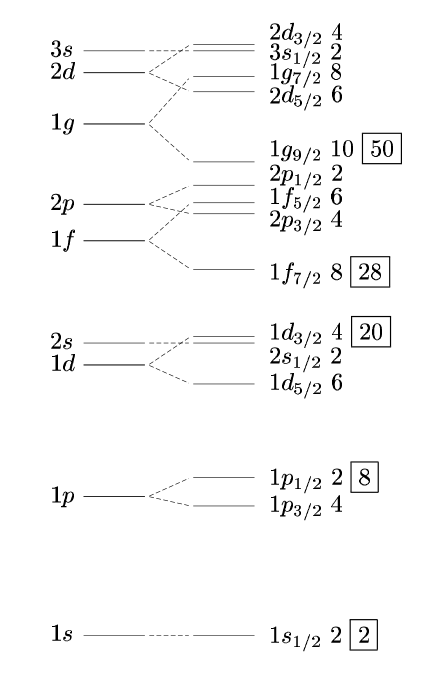
\includegraphics[width=120pt]{fig5_13}
\caption{Struttura delle shell nucleoniche con evidenza sui livelli stabili}
\end{figure}

Quella rappresentata in figura è la schematizzazione dei livelli energetici del nucleo, e si può notare che quindi i nucleoni all'interno del nucleo:
\begin{itemize}
\item non sono posizionati casualmente;
\item hanno momenti angolari;
\item soddisfano la statistica di Fermi e di conseguenza anche al principio di esclusione di Pauli.
\end{itemize}


